% Options for packages loaded elsewhere
\PassOptionsToPackage{unicode}{hyperref}
\PassOptionsToPackage{hyphens}{url}
\PassOptionsToPackage{dvipsnames,svgnames,x11names}{xcolor}
%
\documentclass[
  letterpaper,
  DIV=11,
  numbers=noendperiod]{scrartcl}

\usepackage{amsmath,amssymb}
\usepackage{iftex}
\ifPDFTeX
  \usepackage[T1]{fontenc}
  \usepackage[utf8]{inputenc}
  \usepackage{textcomp} % provide euro and other symbols
\else % if luatex or xetex
  \usepackage{unicode-math}
  \defaultfontfeatures{Scale=MatchLowercase}
  \defaultfontfeatures[\rmfamily]{Ligatures=TeX,Scale=1}
\fi
\usepackage{lmodern}
\ifPDFTeX\else  
    % xetex/luatex font selection
\fi
% Use upquote if available, for straight quotes in verbatim environments
\IfFileExists{upquote.sty}{\usepackage{upquote}}{}
\IfFileExists{microtype.sty}{% use microtype if available
  \usepackage[]{microtype}
  \UseMicrotypeSet[protrusion]{basicmath} % disable protrusion for tt fonts
}{}
\makeatletter
\@ifundefined{KOMAClassName}{% if non-KOMA class
  \IfFileExists{parskip.sty}{%
    \usepackage{parskip}
  }{% else
    \setlength{\parindent}{0pt}
    \setlength{\parskip}{6pt plus 2pt minus 1pt}}
}{% if KOMA class
  \KOMAoptions{parskip=half}}
\makeatother
\usepackage{xcolor}
\setlength{\emergencystretch}{3em} % prevent overfull lines
\setcounter{secnumdepth}{5}
% Make \paragraph and \subparagraph free-standing
\ifx\paragraph\undefined\else
  \let\oldparagraph\paragraph
  \renewcommand{\paragraph}[1]{\oldparagraph{#1}\mbox{}}
\fi
\ifx\subparagraph\undefined\else
  \let\oldsubparagraph\subparagraph
  \renewcommand{\subparagraph}[1]{\oldsubparagraph{#1}\mbox{}}
\fi

\usepackage{color}
\usepackage{fancyvrb}
\newcommand{\VerbBar}{|}
\newcommand{\VERB}{\Verb[commandchars=\\\{\}]}
\DefineVerbatimEnvironment{Highlighting}{Verbatim}{commandchars=\\\{\}}
% Add ',fontsize=\small' for more characters per line
\usepackage{framed}
\definecolor{shadecolor}{RGB}{241,243,245}
\newenvironment{Shaded}{\begin{snugshade}}{\end{snugshade}}
\newcommand{\AlertTok}[1]{\textcolor[rgb]{0.68,0.00,0.00}{#1}}
\newcommand{\AnnotationTok}[1]{\textcolor[rgb]{0.37,0.37,0.37}{#1}}
\newcommand{\AttributeTok}[1]{\textcolor[rgb]{0.40,0.45,0.13}{#1}}
\newcommand{\BaseNTok}[1]{\textcolor[rgb]{0.68,0.00,0.00}{#1}}
\newcommand{\BuiltInTok}[1]{\textcolor[rgb]{0.00,0.23,0.31}{#1}}
\newcommand{\CharTok}[1]{\textcolor[rgb]{0.13,0.47,0.30}{#1}}
\newcommand{\CommentTok}[1]{\textcolor[rgb]{0.37,0.37,0.37}{#1}}
\newcommand{\CommentVarTok}[1]{\textcolor[rgb]{0.37,0.37,0.37}{\textit{#1}}}
\newcommand{\ConstantTok}[1]{\textcolor[rgb]{0.56,0.35,0.01}{#1}}
\newcommand{\ControlFlowTok}[1]{\textcolor[rgb]{0.00,0.23,0.31}{#1}}
\newcommand{\DataTypeTok}[1]{\textcolor[rgb]{0.68,0.00,0.00}{#1}}
\newcommand{\DecValTok}[1]{\textcolor[rgb]{0.68,0.00,0.00}{#1}}
\newcommand{\DocumentationTok}[1]{\textcolor[rgb]{0.37,0.37,0.37}{\textit{#1}}}
\newcommand{\ErrorTok}[1]{\textcolor[rgb]{0.68,0.00,0.00}{#1}}
\newcommand{\ExtensionTok}[1]{\textcolor[rgb]{0.00,0.23,0.31}{#1}}
\newcommand{\FloatTok}[1]{\textcolor[rgb]{0.68,0.00,0.00}{#1}}
\newcommand{\FunctionTok}[1]{\textcolor[rgb]{0.28,0.35,0.67}{#1}}
\newcommand{\ImportTok}[1]{\textcolor[rgb]{0.00,0.46,0.62}{#1}}
\newcommand{\InformationTok}[1]{\textcolor[rgb]{0.37,0.37,0.37}{#1}}
\newcommand{\KeywordTok}[1]{\textcolor[rgb]{0.00,0.23,0.31}{#1}}
\newcommand{\NormalTok}[1]{\textcolor[rgb]{0.00,0.23,0.31}{#1}}
\newcommand{\OperatorTok}[1]{\textcolor[rgb]{0.37,0.37,0.37}{#1}}
\newcommand{\OtherTok}[1]{\textcolor[rgb]{0.00,0.23,0.31}{#1}}
\newcommand{\PreprocessorTok}[1]{\textcolor[rgb]{0.68,0.00,0.00}{#1}}
\newcommand{\RegionMarkerTok}[1]{\textcolor[rgb]{0.00,0.23,0.31}{#1}}
\newcommand{\SpecialCharTok}[1]{\textcolor[rgb]{0.37,0.37,0.37}{#1}}
\newcommand{\SpecialStringTok}[1]{\textcolor[rgb]{0.13,0.47,0.30}{#1}}
\newcommand{\StringTok}[1]{\textcolor[rgb]{0.13,0.47,0.30}{#1}}
\newcommand{\VariableTok}[1]{\textcolor[rgb]{0.07,0.07,0.07}{#1}}
\newcommand{\VerbatimStringTok}[1]{\textcolor[rgb]{0.13,0.47,0.30}{#1}}
\newcommand{\WarningTok}[1]{\textcolor[rgb]{0.37,0.37,0.37}{\textit{#1}}}

\providecommand{\tightlist}{%
  \setlength{\itemsep}{0pt}\setlength{\parskip}{0pt}}\usepackage{longtable,booktabs,array}
\usepackage{calc} % for calculating minipage widths
% Correct order of tables after \paragraph or \subparagraph
\usepackage{etoolbox}
\makeatletter
\patchcmd\longtable{\par}{\if@noskipsec\mbox{}\fi\par}{}{}
\makeatother
% Allow footnotes in longtable head/foot
\IfFileExists{footnotehyper.sty}{\usepackage{footnotehyper}}{\usepackage{footnote}}
\makesavenoteenv{longtable}
\usepackage{graphicx}
\makeatletter
\def\maxwidth{\ifdim\Gin@nat@width>\linewidth\linewidth\else\Gin@nat@width\fi}
\def\maxheight{\ifdim\Gin@nat@height>\textheight\textheight\else\Gin@nat@height\fi}
\makeatother
% Scale images if necessary, so that they will not overflow the page
% margins by default, and it is still possible to overwrite the defaults
% using explicit options in \includegraphics[width, height, ...]{}
\setkeys{Gin}{width=\maxwidth,height=\maxheight,keepaspectratio}
% Set default figure placement to htbp
\makeatletter
\def\fps@figure{htbp}
\makeatother

\KOMAoption{captions}{tableheading}
\makeatletter
\makeatother
\makeatletter
\makeatother
\makeatletter
\@ifpackageloaded{caption}{}{\usepackage{caption}}
\AtBeginDocument{%
\ifdefined\contentsname
  \renewcommand*\contentsname{Table of contents}
\else
  \newcommand\contentsname{Table of contents}
\fi
\ifdefined\listfigurename
  \renewcommand*\listfigurename{List of Figures}
\else
  \newcommand\listfigurename{List of Figures}
\fi
\ifdefined\listtablename
  \renewcommand*\listtablename{List of Tables}
\else
  \newcommand\listtablename{List of Tables}
\fi
\ifdefined\figurename
  \renewcommand*\figurename{Figure}
\else
  \newcommand\figurename{Figure}
\fi
\ifdefined\tablename
  \renewcommand*\tablename{Table}
\else
  \newcommand\tablename{Table}
\fi
}
\@ifpackageloaded{float}{}{\usepackage{float}}
\floatstyle{ruled}
\@ifundefined{c@chapter}{\newfloat{codelisting}{h}{lop}}{\newfloat{codelisting}{h}{lop}[chapter]}
\floatname{codelisting}{Listing}
\newcommand*\listoflistings{\listof{codelisting}{List of Listings}}
\makeatother
\makeatletter
\@ifpackageloaded{caption}{}{\usepackage{caption}}
\@ifpackageloaded{subcaption}{}{\usepackage{subcaption}}
\makeatother
\makeatletter
\@ifpackageloaded{tcolorbox}{}{\usepackage[skins,breakable]{tcolorbox}}
\makeatother
\makeatletter
\@ifundefined{shadecolor}{\definecolor{shadecolor}{rgb}{.97, .97, .97}}
\makeatother
\makeatletter
\makeatother
\makeatletter
\makeatother
\ifLuaTeX
  \usepackage{selnolig}  % disable illegal ligatures
\fi
\IfFileExists{bookmark.sty}{\usepackage{bookmark}}{\usepackage{hyperref}}
\IfFileExists{xurl.sty}{\usepackage{xurl}}{} % add URL line breaks if available
\urlstyle{same} % disable monospaced font for URLs
\hypersetup{
  pdftitle={Getting Started with RStudio},
  pdfauthor={Justin Baumann},
  colorlinks=true,
  linkcolor={blue},
  filecolor={Maroon},
  citecolor={Blue},
  urlcolor={Blue},
  pdfcreator={LaTeX via pandoc}}

\title{Getting Started with RStudio}
\author{Justin Baumann}
\date{}

\begin{document}
\maketitle
\ifdefined\Shaded\renewenvironment{Shaded}{\begin{tcolorbox}[sharp corners, frame hidden, boxrule=0pt, interior hidden, borderline west={3pt}{0pt}{shadecolor}, breakable, enhanced]}{\end{tcolorbox}}\fi

\renewcommand*\contentsname{Table of contents}
{
\hypersetup{linkcolor=}
\setcounter{tocdepth}{3}
\tableofcontents
}
\hypertarget{learning-objectives}{%
\section{\texorpdfstring{\textbf{Learning
Objectives}}{Learning Objectives}}\label{learning-objectives}}

IN THIS TUTORIAL YOU WILL LEARN:\\
1.) How to access and/or install R and RStudio\\
2.) How to navigate RStudio\\
3.) How to set and change the working directory\\
4.) How to setup an RStudio Project

\hypertarget{additional-tutorials-and-resources}{%
\section{Additional Tutorials and
Resources}\label{additional-tutorials-and-resources}}

\href{https://www.datacamp.com/community/tutorials/tidyverse-tutorial-r}{Datacamp
Tidyverse tutorial}

\href{https://www.tidyverse.org/learn/}{Books and workshops for learning
tidyverse}

\href{https://and.netlify.app/tutorials/02/}{A nice step by step
walkthough of Tidyverse functions}

\href{https://www.youtube.com/watch?v=JtQfXY0lIzc}{Video Tidyverse
tutorial}

\href{https://rstudio.cloud/learn/primers}{Want to TRY some stuff on
your own? Use the RStudio.cloud primers}

The best way to learn is to GOOGLE IT and try stuff

\begin{center}\rule{0.5\linewidth}{0.5pt}\end{center}

\hypertarget{install-r-and-rstudio-and-access-the-rstudio-server}{%
\section{\texorpdfstring{\textbf{1.) Install R and RStudio and access
the Rstudio
server}}{1.) Install R and RStudio and access the Rstudio server}}\label{install-r-and-rstudio-and-access-the-rstudio-server}}

In this course we will learn how to program in R (a coding language)
using RStudio (a coding environment). RStudio makes using R easier and
more user friendly!\\
We will also learn how to make pdf and html output files that include
code and outputs (tables and graphs).\\
These are handy tools for reporting data and even for writing papers! We
will use Quarto to do this (a new tool from the folks who designed
RStudio).\\
Your lab reports will all be built using Quarto.

\textbf{You have options:}\\
1. Install R and RStudio on your device(s) and use it locally\\
2. Sign up for a posit cloud account here:
https://posit.cloud/plans/free. Posit Cloud is a way to access RStudio
online without downloading and installing anything. If you are a
student, faculty, or staff at a college or university, your school may
have an RStudio server. Mount Holyoke has one, for example. You can
access it for free (if you are an affiliate) at
https://rstudio.mtholyoke.edu/. Note that for the rstudio.mtholyoke.edu
website to work you need to login AND you must either be on campus or be
using the MHC VPN.\\

\subsection{\texorpdfstring{\textbf{Install R}}{Install R}}

To install R, we will use this link:
\href{https://cran.r-project.org/bin/}{install R}\\
1.) Choose the operating system you use (macosx or windows)\\
2.) Click the blue .pkg link that aligns with your computer and
operating system (ask questions if needed)\\
3.) Follow instructions

\subsection{\texorpdfstring{\textbf{Install RStudio}}{Install RStudio}}

1.) Click
\href{https://www.rstudio.com/products/rstudio/download/\#download}{this
link} and follow instructions\\
2.) OPEN RStudio (not R). Click on the logo that is a white R inside a
blue circle (RStudio). We never need to open R, we can use RStudio.

\subsection{\texorpdfstring{\textbf{Access the MHC
Server}}{Access the MHC Server}}

1.) follow this link
\href{https://rstudio.mtholyoke.edu}{rstudio.mtholyoke.edu}\\
2.) login\\
3.) This is RStudio hosted by Mt Holyoke servers. It requires 2 things:
a.) internet connection b.) you must be on campus OR you must have the
Mt Holyoke VPN activated. To learn about the VPN, check out
\href{https://lits.mtholyoke.edu/tech-support/access-and-internet-connectivity/connect-campus/using-virtual-private-network-vpn}{this
page}

\begin{center}\rule{0.5\linewidth}{0.5pt}\end{center}

\hypertarget{rstudio-layout}{%
\section{\texorpdfstring{\textbf{2.) RStudio
Layout}}{2.) RStudio Layout}}\label{rstudio-layout}}

\subsection{\texorpdfstring{\textbf{Top Left}:
Script}{Top Left: Script}}

Where you will write your script(s). This is where we should be writing
our code! It can be run, commented, and saved here.

\subsection{\texorpdfstring{\textbf{Bottom Left}:
Console/terminal}{Bottom Left: Console/terminal}}

Here you can run single lines of code and/or see error messages,
warnings, and other outputs. Code should not be written here unless it
is simple / for testing! Anything worth keeping should go in the script
at the top left!

\subsection{\texorpdfstring{\textbf{Top Right}: Environment, History,
etc\ldots{}}{Top Right: Environment, History, etc\ldots{}}}

Here you will be able to see the dataframes you have read into R or
created (using the ``Environment tab''). The other tabs are less useful
for us at this stage, but feel free to explore them! Note: The Broom
icon can be used to clear dataframes from your environment. You can
minimize or maximize this and each other quadrant using the symbols at
the top right of the quadrant (a collapsed page next to a full page)

\subsection{\texorpdfstring{\textbf{Bottom Right}: Files, Plots,
Packages,
etc\ldots{}}{Bottom Right: Files, Plots, Packages, etc\ldots{}}}

This is the second most important quadrant (behind top left) and we can
change the working directory here very easily. Here we can see the files
in our present working directory (we will learn about that next!) We can
also see any plots we make in the plots tab. VERY importantly, we can
see the packages we have loaded or installed in the packages tab. This
will be useful to you! You can also use this tab to search the internal
Help dictionary, though I will note that the internet is often more
helpful!

\subsection{\texorpdfstring{\textbf{Top Bar}: File, Edit,
Etc\ldots{}}{Top Bar: File, Edit, Etc\ldots{}}}

You can use the top bar in RStudio much like in any other program. I'll
let you explore that on your own. Notably, in the top right corner of
the top bar you will see an `R' in a blue box. This is where you can set
the project you are working form. Using projects is great because it
allows you an easy way to compartmentalize your code, data, figures, and
working directory for a single project all in one place! We will get to
this shortly.

\hypertarget{section}{%
\section*{}\label{section}}
\addcontentsline{toc}{section}{}

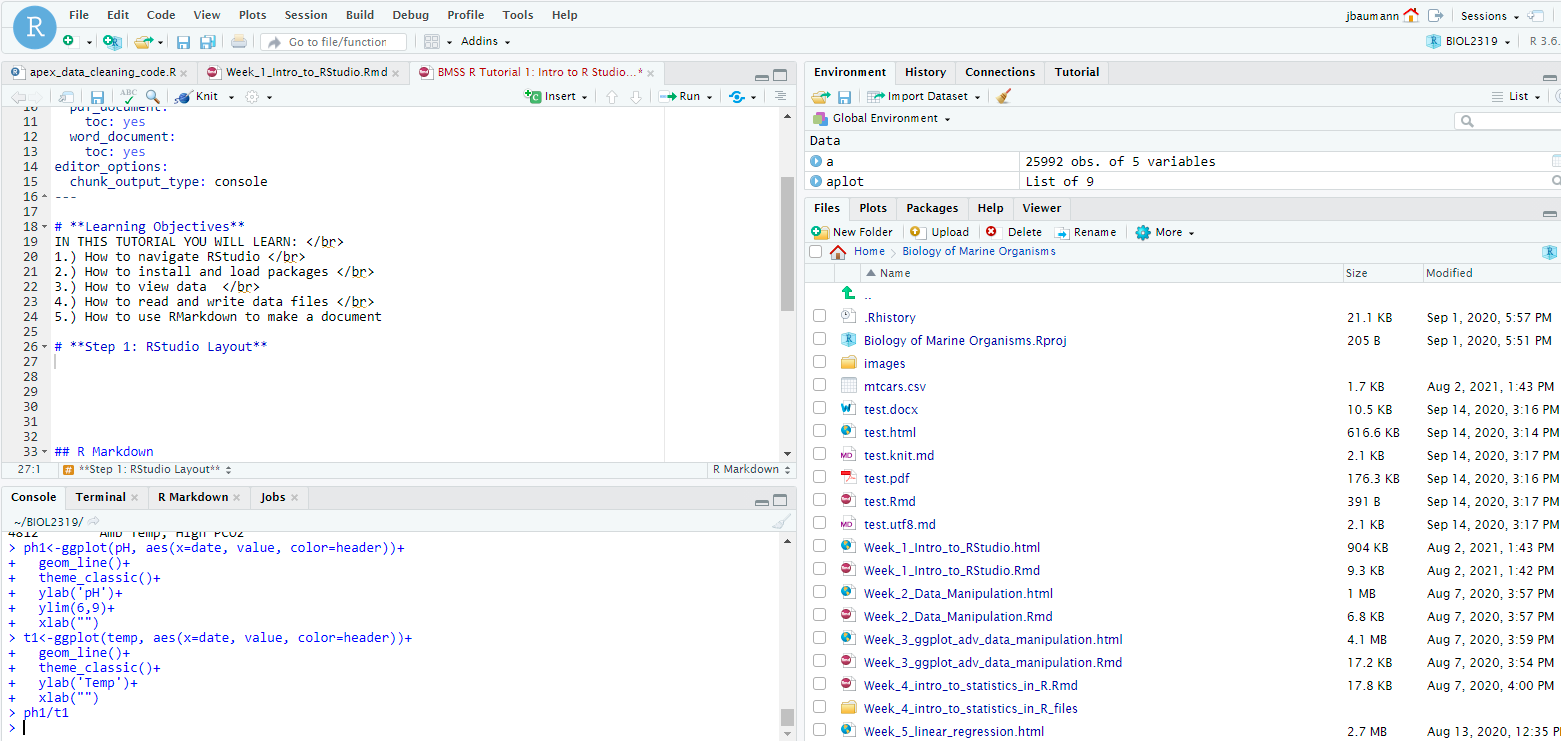
\includegraphics{images/RStudio_layout.png}

\begin{center}\rule{0.5\linewidth}{0.5pt}\end{center}

\hypertarget{the-working-directory---what-is-it-how-to-check-it-and-how-to-set-it}{%
\section{\texorpdfstring{\textbf{3.) The Working Directory} - What is
it, how to check it, and how to set
it!}{3.) The Working Directory - What is it, how to check it, and how to set it!}}\label{the-working-directory---what-is-it-how-to-check-it-and-how-to-set-it}}

1.) We can use the getwd() command!

\begin{Shaded}
\begin{Highlighting}[]
\FunctionTok{getwd}\NormalTok{()}
\end{Highlighting}
\end{Shaded}

\begin{verbatim}
[1] "C:/Users/Justin Baumann/Desktop/r_for_bioeco/intro_r_for_bio_eco"
\end{verbatim}

2.) We can also use the Bottom Right ``Files'' tab

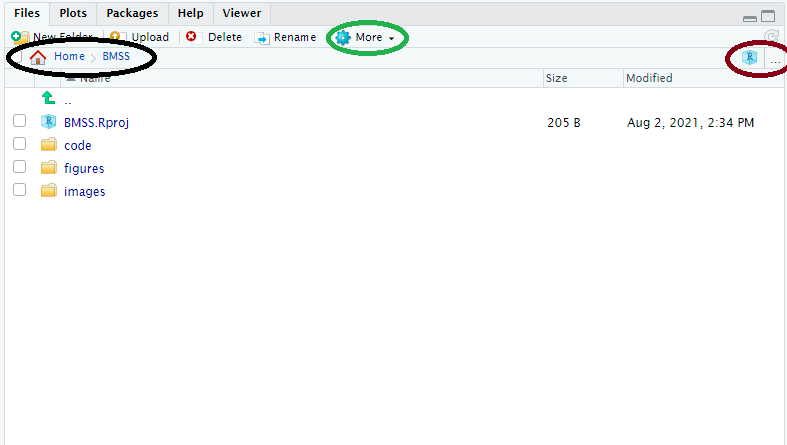
\includegraphics{images/files.png}

Here our working directory (and it's file path) can be located in the
black circle. We can manually change the working directory by using the
`\ldots{}' in the brown circle to find any folder on our computer (or
attached cloud folders), navigating to it, and then using the `More' Cog
in the green circle to ``Set as working directory''

3.) An alternative approach to finding the working directory in the
``Files'' tab. Using the ``More'' cog, we can select ``Go to working
directory''

\hypertarget{how-to-set-the-working-directory}{%
\subsection{\texorpdfstring{\textbf{How to SET the working
directory}}{How to SET the working directory}}\label{how-to-set-the-working-directory}}

1.) Using the ``Files'' tab to set manually: a.) Using the `\ldots{}' in
the `Files' tab you can select any directory (folder) on your computer.
You can also set a google drive, box, dropbox, or other shared folder as
your working directory if you'd like (as long as you are syncing a
folder between the cloud and your computer -- ASK me if you have
questions about this!) b.) Once you navigate to a directory you still
need to \textbf{SET IT} as your working directory. You do this in the
``More'' cog-- select ``Set as working directory''

2.) Set working directory with code: We use the `setwd()' function for
this. Below is an example. You will need to replace the path details
with your own!

\begin{Shaded}
\begin{Highlighting}[]
\FunctionTok{setwd}\NormalTok{(}\StringTok{"C:/Users/Justin Baumann/Desktop/BIOL234\_Biostats\_MHC/Spring 2023/Labs"}\NormalTok{)}
\end{Highlighting}
\end{Shaded}

\hypertarget{rstudio-projects}{%
\section{\texorpdfstring{\textbf{3.) RStudio
Projects!}}{3.) RStudio Projects!}}\label{rstudio-projects}}

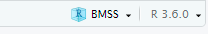
\includegraphics{images/projects.png}\\

RStudio Projects are a great way to compartmentalize your coding work!
You can store your code, outputs, input files, figures, etc all in one
directory (with subdirectories). When you load your R Project, R will
automatically load the last scripts you were working with on that
project as well as the dataframes and items you have read in (your
environment will be ready to go!). It will also navigate to the correct
working directory automatically :) This will make your life easier!

\emph{To make an RStudio Project}\\
1.) Create a folder on your computer (or cloud storage) that will serve
as the MAIN directory for your project. Within that folder I recommend
you make subdirectories for all of your R related inputs and outputs.
Maybe something like I have here:

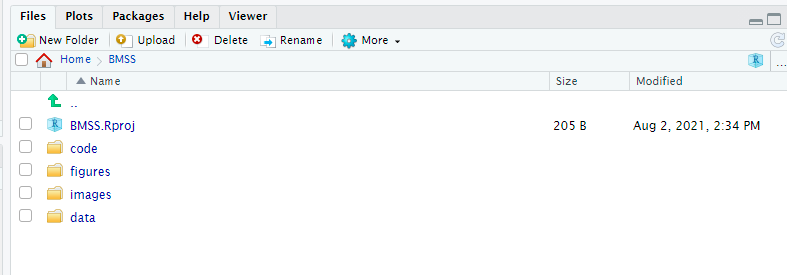
\includegraphics{images/projectex.png}

2.) Once you have a MAIN directory folder created (whether you've made
subdirectories or not) you can create a project! Set your main folder as
your working directory. Next, navigate to the TOP RIGHT of your screen
and select the down arrow next to the Big ``R'' in a blue box. NOW,
select ``New Project'' --\textgreater{} Existing directory
--\textgreater{} Name the project and hit done! At this point you will
see a .Rproj file appear in your MAIN directory. This means you did it
right :) This .Rproj file is how you save all of your project info. It
autosaves and when you select your project (Again, TOP RIGHT of your
screen, select the down arrow next to the R in the blue box and then
select your project name) it will load up your scripts, environment, and
set your working directory as the MAIN folder. You can navigate VERY
easily from here :)

\begin{center}\rule{0.5\linewidth}{0.5pt}\end{center}



\end{document}
